% tikzpic.tex
\documentclass[crop,tikz]{standalone}% 'crop' is the default for v1.0, before it was 'preview'
%\usetikzlibrary{...}% tikz package already loaded by 'tikz' option
\usepackage{amsmath,amsthm,amssymb,mathrsfs,amsfonts,dsfont}

\begin{document}
    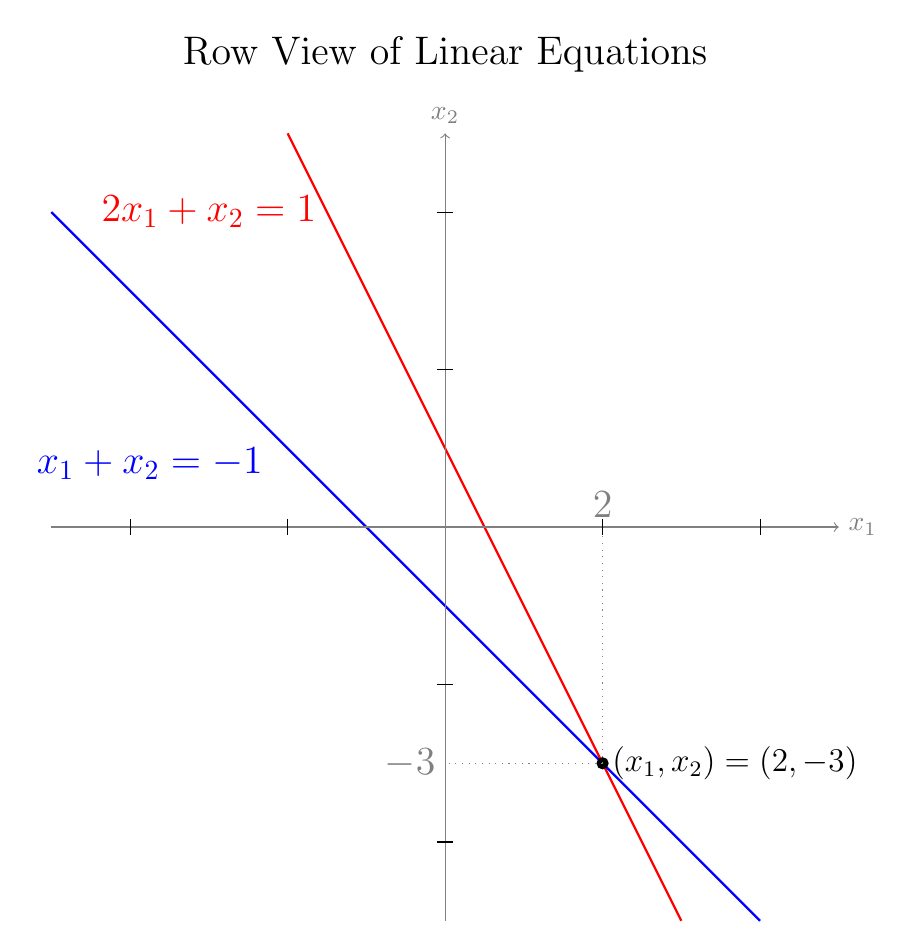
\begin{tikzpicture}[scale=1.0]
        % Text title saying "Row View"
        \node[font=\Large] at (0, 6) {Row View of Linear Equations};

        % Write down equation1.
        \node[font=\Large, red] at (-3, 4) {$2x_1 + x_2 = 1$};
        % Draw the line 2x1 + x2 = 1 in red and blue within the coordinate systems with x and y between -5 and 5.
        \draw[red, thick] (-2, 5) -- (3, -5);
        
        \node[font=\Large, blue] at (-3.75, 0.8) {$x_1 + x_2 = -1$};
        % Draw the line x1 + x2 = 1 in red and blue within the coordinate systems with x and y between -5 and 5.
        \draw[blue, thick] (-5, 4) -- (4, -5);

        % Plot the point of intersection by a filled circle.
        \filldraw[black] (2, -3) circle (2pt) node[font=\large, anchor=west] {$(x_1, x_2) = (2, -3)$};
        % Dotted lines to the coordinate axes.
        \draw[dotted, gray] (2, -3) -- (2, 0) node[font=\Large, anchor=south] {$2$};
        \draw[dotted, gray] (2, -3) -- (0, -3) node[font=\Large, anchor=east] {$-3$};
    
        \draw[->, gray] (-5,0) -- (5,0) node[right] {$x_1$};
        \draw[->, gray] (0,-5) -- (0,5) node[above] {$x_2$};
        \foreach \x in {-4,-2,2,4}
        \draw (\x,0.1) -- (\x,-0.1);
        \foreach \y in {-4,-2,2,4}
        \draw (0.1,\y) -- (-0.1,\y);
    \end{tikzpicture}
\end{document}